%!TEX root =  ../paper.tex
\section{Intel SGX Background}
\label{ch:background:SGX}

Intel SGX is a TEE architecture that isolates application enclaves from all other software running on the system, including the privileged OS, hypervisor, BIOS etc.~\cite{sgxexplained}. Enclave's data is encrypted and integrity protected whenever it is moved outside the CPU chip. The untrusted OS is responsible for the enclave creation and its initialization actions are recorded securely inside the CPU, creating a \emph{measurement} that captures the enclave's code. Enclaves can perform local attestation, which allows one enclave to ask the CPU to generate a signed report that includes its measurement. Another enclave on the same platform can verify the validity of the report without interacting with any other external services. Enclaves can \emph{seal} data to disk, which  allows them to securely store confidential data such  that only the same enclave running in the same CPU will be able to retrieve it later.



\subsection{Attestation}

Attestation is an important security primitive for a TEE that ensures that the SGX platform is running a proper piece of software (enclave). Upon instantiation by the trusted hardware, the platform can compute the \emph{measurement} of the enclave that includes the cryptographic hash of the code, data, stack, heap etc. The measurement of the enclave is then signed by the platform's private key. This signed measurement is known as the report. A verifier can then check the signature of the report to verify the following:

\begin{enumerate}
  \item The enclave is running on a legitimate platform.
  \item The enclave code is proper as it matches a known measurement of the software.
  \item Corresponding public key of the platform to create a secure channel with the enclave in order to provision secret to that enclave.
\end{enumerate}  

Intel SGX also implements an attestation scheme which follows the same principles. Every Intel processor comes with two device root key that fused into the processor during the production phase~\cite{attestation_primitive} -  root provisioning key and root sealing key. These keys are the related key generations are shown in Figure~\ref{fig:keys_bg}. The attestation key is derived from these initial platform keys that are used to generate report from the enclave measurement.


\begin{figure}[t]
  \centering
    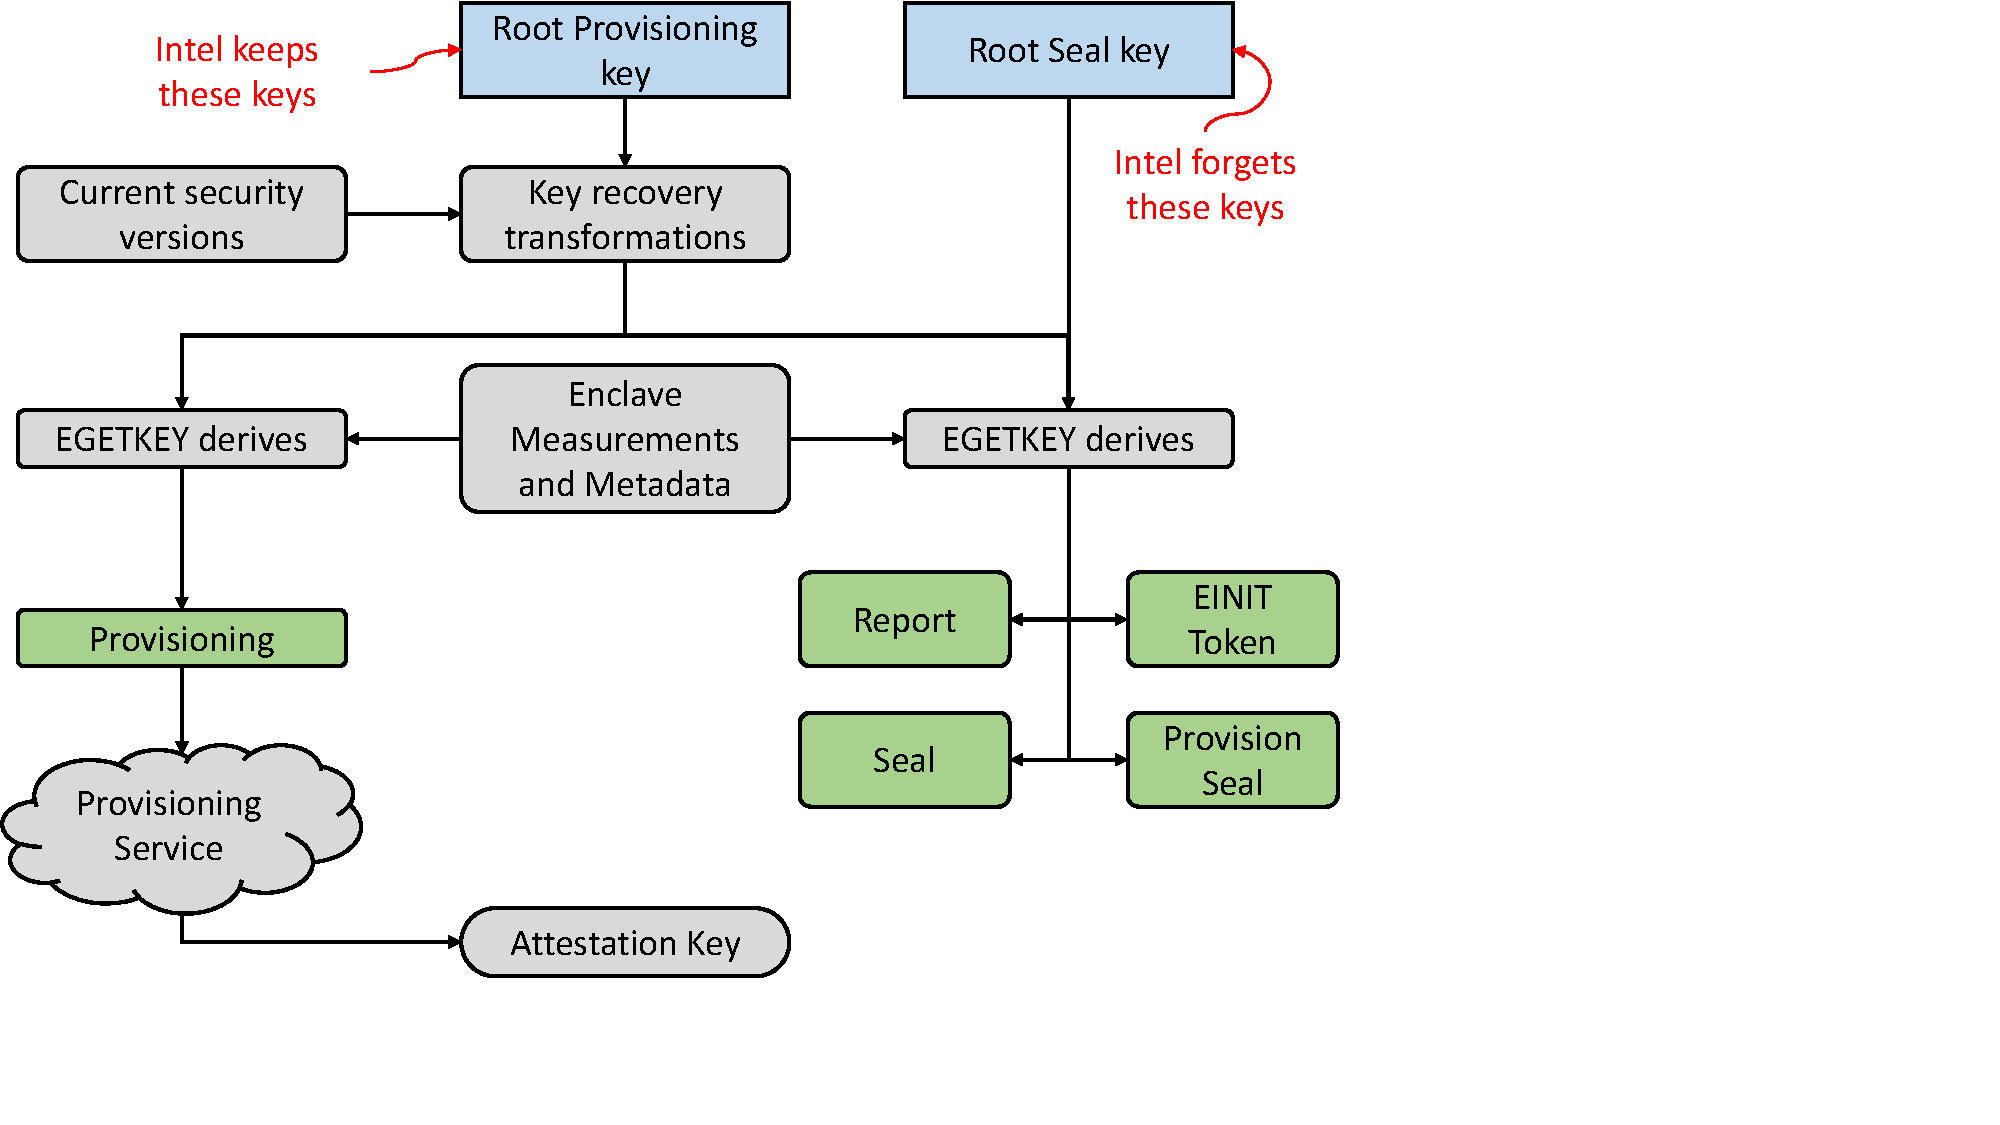
\includegraphics[trim={0 1cm 10cm 0},clip,width=0.9\linewidth]{chapters/background/figures/keys.pdf}
    \caption[Intel SGX keys and key derivations]{\textbf{Intel SGX keys and key derivations.} }
    \label{fig:keys_bg}
\end{figure}


\myparagraph{Measurement} When an enclave is built and initialized, Intel SGX will generate a cryptographic log of all the build activities (details in~\cite{attestation_primitive_all}), including:

\begin{itemize}
  \item Content: code, data, stack, heap
  \item Location of each page within the enclave
  \item Security flags being used
\end{itemize}
    
The ``Enclave Identity'', which is a 256-bit hash digest of the log, is stored as \texttt{MRENCLAVE} as the enclave�s software TCB. In order to verify the software TCB, one should first securely obtain the enclave�s software TCB, then securely obtain the expected enclave�s software TCB and compare those two values.

\myparagraph{Report} \texttt{REPORT} contains the following information:

\begin{itemize}
  \item Measurement of the code and data in the enclave.
  \item A hash of the public key in the ISV certificate presented at enclave initialization time.
  \item User data.
  \item Other security related state information.
  \item A signature block over the above data, which can be verified by the same platform that produced the report.
\end{itemize}

Intel SGX supports both local and remote attestation. In this chapter, we only describe remote attestation as this form of attestation is the most relevant.


\subsection{Remote Attestation}
\label{ch:background:SGX:remote}

Remote attestation enables an external verifier to check whether a specific enclave has been correctly instantiated in a SGX protected environment. In the following, we describe the two main classes of remote attestation supported by Intel: i) ``enhanced privacy ID'' (EPID) attestation~\cite{epid_attestation}, and ii) the recently introduced ``data center attestation primitives'' (DCAP)~\cite{DCAP}.

\myparagraph{EPID attestation}
The EPID remote attestation is an interactive protocol between three parties: the remote verifier; the attested SGX platform; and the Intel Attestation Service (IAS), an online service operated by Intel. 
Each SGX platform includes a system service called \emph{Quoting Enclave} (QE) that has exclusive access to an attestation key. The remote verifier sends a random challenge to the attested platform, which replies with a QUOTE structure, capturing the enclave's measurement from its creation, signed with the attestation key. The verifier can then send the QUOTE to the IAS that verifies its signature and correctness, checks that the attestation key has not been revoked, and in case of successful attestation signs the QUOTE. 

The attestation key used by the QE is part of a group signature scheme called EPID that supports two signature modes: random base mode and name base mode, also called ``linkable'' mode. Both signature modes do not uniquely identify the processor to the IAS; but only a group, like a particular processor manufacturing batch. The difference between them is that the linkable signature mode allows to check whether two attestation requests came from the same CPU. 


\myparagraph{DCAP attestation} Whereas the EPID attestation variant requires connectivity to an Intel-operated attestation service, and is limited to pre-defined signature algorithms, the main goal of the DCAP attestation variant is to enable corporations to run their own local attestation services with freely chosen signature types. To achieve this, each SGX platforms is, at the time of manufacturing, equipped with a unique \emph{Platform Provisioning ID} (PPID) and \emph{Provisioning Certification Key} (PCK). Intel also provides a trusted \emph{Provisioning Certification Enclave} (PCE) that acts as a local CA and certifies custom Quoting Enclaves that can use freely-chosen attestation services and signatures.

DCAP attestation requires a trusted enrollment phase, where the enrolled SGX platform sends its PPID (in encrypted format) to a local corporate key management system that obtains a PCK certificate for the enrolled platform from an Intel-operated DCAP service. After that, the custom Quoting Enclave can create a new attestation key that is certified by the PCE enclave on the same platform. The certified attestation key can then be delivered to the corporate key management system that verifies it using the previously obtained PCK certificate. Once such enrollment phase is complete, the custom QE can sign attestation statements that can be verified by a local corporate attestation service without contacting Intel.



\subsection{Side-Channel Leakage}
\label{sec:background:attacks}

Recent research has demonstrated that the SGX architecture is susceptible to side-channel leakage. Secret-dependent data and code access patterns can be observed by monitoring shared physical resources such as CPU caches~\cite{sgxcache,gotzfried2017cache,moghimi2017cachezoom} or the branch prediction unit~\cite{lee2017inferring}. The OS can also infer enclave's execution control flow or data accesses by monitoring page fault events~\cite{xu2015controlled}. Many such attacks can be addressed by hardening the enclave's code, e.g., using cryptographic implementations where the data or code access patterns are independent of the key.

The recently discovered system vulnerabilities Spectre~\cite{Kocher2018spectre} and Meltdown~\cite{Lipp2018meltdown} allow application-level code to read memory content of privileged processes across separation boundaries by exploiting subtle side-effects of transient execution. The Foreshadow attack~\cite{foreshadow-usenix18} demonstrates how to extract SGX attestation keys from processors by leveraging the Meltdown vulnerability. 

\subsection{Microcode updates}
During manufacturing, each SGX processor is equipped with hardware keys. When SGX software is installed on the CPU for the first time, the platform runs a provisioning protocol with Intel. In this protocol, the platform uses one of the hardware keys to demonstrates that it is a genuine Intel CPU running a specific microcode version and it then then joins a matching EPID group and obtains an attestation key~\cite{epid_attestation} (or a signing key for the PCE enclave). 

Microcode patches issued by Intel can be installed to processors that are affected by known vulnerabilities such as the above mentioned Foreshadow attack. When a new microcode version is installed, the processor repeats the provisioning procedure and joins a new group that corresponds to the updated microcode version and obtains a new attestation key which allows IAS to distinguish attestation signatures that originate from patched processors from attestation signatures made by unpatched processors~\cite{epid_attestation}.